\documentclass[crop,tikz,border=8pt]{standalone}
\usepackage[utf8]{inputenc}
\usetikzlibrary{positioning,calc}

\begin{document}
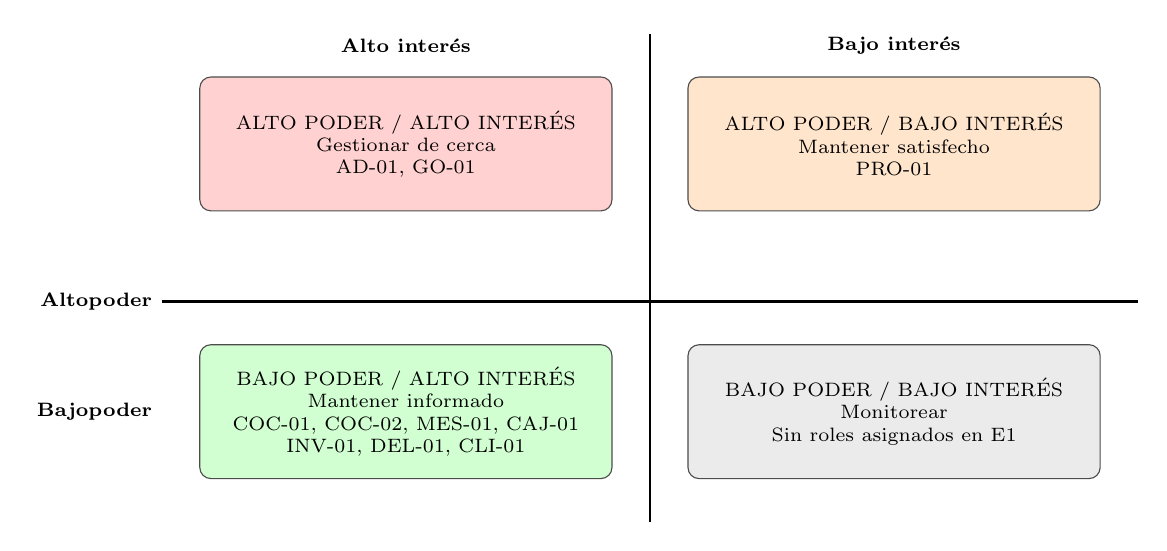
\begin{tikzpicture}[
  q/.style={draw=black!70,rounded corners,align=center,text width=5.0cm,
            minimum height=1.7cm,font=\scriptsize},
  ax/.style={font=\scriptsize\bfseries}
]
\node[q,fill=red!18] (q1) at (0,2.0) {ALTO PODER / ALTO INTERÉS\\Gestionar de cerca\\
{\scriptsize AD-01, GO-01}};
\node[q,fill=orange!20] (q2) at (6.2,2.0) {ALTO PODER / BAJO INTERÉS\\Mantener satisfecho\\
{\scriptsize PRO-01}};
\node[q,fill=green!18] (q3) at (0,-1.4) {BAJO PODER / ALTO INTERÉS\\Mantener informado\\
{\scriptsize COC-01, COC-02, MES-01, CAJ-01\\INV-01, DEL-01, CLI-01}};
\node[q,fill=gray!16] (q4) at (6.2,-1.4) {BAJO PODER / BAJO INTERÉS\\Monitorear\\
{\scriptsize Sin roles asignados en E1}};

\draw[thick] (-3.1,0) -- (9.3,0);
\draw[thick] (3.1,-2.8) -- (3.1,3.4);
\node[ax,left] at (-3.1,0) {Alto\\poder};
\node[ax,left] at (-3.1,-1.4) {Bajo\\poder};
\node[ax] at (0,3.25) {Alto interés};
\node[ax] at (6.2,3.25) {Bajo interés};
\end{tikzpicture}
\end{document}
